%-------------------------------------------------------------------------------
% Fichero:	
% Documento:	Presentación para el taller "SODAR: Iniciación a Arduino + Processing"
% Autores:	
% Fecha:        
% Descripción:	La presentación del taller
% Versión:      0.00
% Historial:    0.00 
%-------------------------------------------------------------------------------

\documentclass{beamer}

\mode<presentation>
{
  \usetheme{Warsaw}
  \usecolortheme[RGB={52,170,205}]{structure}
  \setbeamertemplate{navigation symbols}{}
}
\DeclareGraphicsExtensions{.pdf,.png,.jpg} %solo para PDFLaTeX
\graphicspath{{figures/}{graphics/}{images/}}

% Esto es para poder escribir acentos directamente:
\usepackage[utf8]{inputenc}
% Esto es para que el LaTeX sepa que el texto está en español:
\usepackage[spanish]{babel}

\usepackage{bookman}
\usepackage{eurosym}

% \usepackage{times}
% \usepackage[T1]{fontenc}
% Or whatever. Note that the encoding and the font should match. If T1
% does not look nice, try deleting the line with the fontenc.

\title[Taller SODAR] % (optional, use only with long paper titles)
{SODAR: Iniciación a Arduino + Processing}

\subtitle
{Un taller BricoLabs} % (optional)

\author[ctemes, eukelade, milo, salvari] % (optional, use only with lots of authors)
{ctemes \and eukelade \and Milo \and salvari}
% - Use the \inst{?} command only if the authors have different
%   affiliation.

\institute[BricoLabs] % (optional, but mostly needed)
{
Asociación BricoLabs 
}
% - Use the \inst command only if there are several affiliations.
% - Keep it simple, no one is interested in your street address.

\date[Short Occasion] % (optional)
{7 noviembre / OSHWDem - 2014}

\subject{Taller Arduino Processing}
% This is only inserted into the PDF information catalog. Can be left
% out. 



% If you have a file called "university-logo-filename.xxx", where xxx
% is a graphic format that can be processed by latex or pdflatex,
% resp., then you can add a logo as follows:

\pgfdeclareimage[height=0.4cm]{oshwdem-logo}{OSHWIcolor.png}
% \logo{\pgfuseimage{oshwdem-logo}}




% Delete this, if you do not want the table of contents to pop up at
% the beginning of each subsection:
\AtBeginSubsection[]
{
  \begin{frame}<beamer>{Agenda}
    \tableofcontents[currentsection,currentsubsection]
  \end{frame}
}


% If you wish to uncover everything in a step-wise fashion, uncomment
% the following command: 

%\beamerdefaultoverlayspecification{<+->}


\begin{document}

\begin{frame}
  \titlepage
\end{frame}

\begin{frame}{Agenda}
  \tableofcontents
  % You might wish to add the option [pausesections]
\end{frame}


% Since this a solution template for a generic talk, very little can
% be said about how it should be structured. However, the talk length
% of between 15min and 45min and the theme suggest that you stick to
% the following rules:  

% - Exactly two or three sections (other than the summary).
% - At *most* three subsections per section.
% - Talk about 30s to 2min per frame. So there should be between about
%   15 and 30 frames, all told.

\section{Presentación}
\subsection{¿Quienes somos?}

\begin{frame}{BricoLabs y la OSHWDem}

LOGOS BL Y OSHWI Y DOS FOTOS   
\end{frame}


\begin{frame}{Ponentes}
  \begin{itemize}
  \item Carlos Temes
  \item Eukelade
  \item Milo
  \item Salvari
  \end{itemize}
\end{frame}

\begin{frame}{Asistentes}
  \begin{itemize}
  \item ¿Quién conoce el Arduino?
    \pause
  \item ¿Quién conoce Processing?
    \pause
  \item ¿Traéis los deberes hechos? ;)
  \end{itemize}
\end{frame}

\subsection{Requisitos}

\begin{frame}{Revisar la instalación}
  Cargar el blink de ejemplo en Arduino
\end{frame}

\section{Arduino}
\subsection{Intro}
\begin{frame}{SODAR}

FOTO DEL MONTAJE
  
\end{frame}

\begin{frame}{Arduino}

  \begin{figure}
    \centering
%    \caption{IuCS}
%    \label{fig:estruct}
    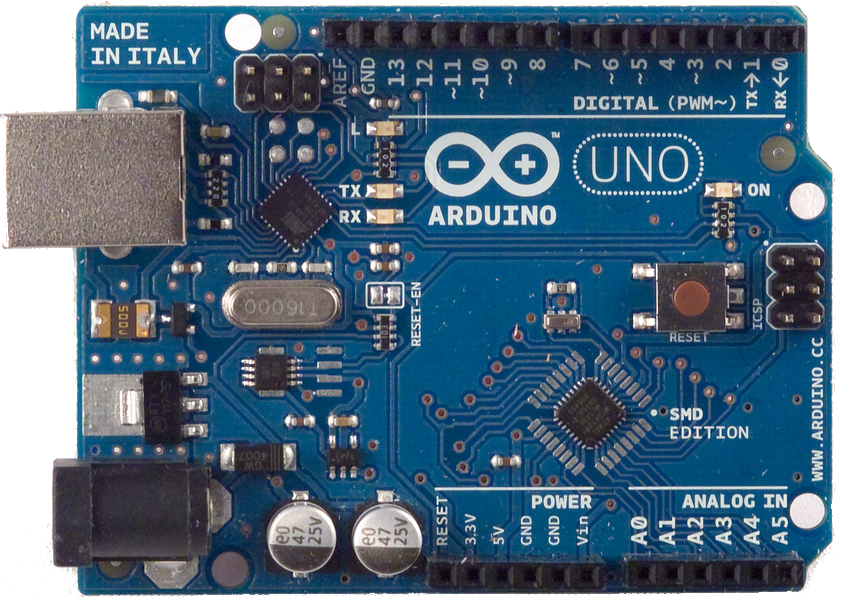
\includegraphics [width=0.7\textwidth]{ArduinoUnoSmd.jpg}
  \end{figure}


  Link a la página oficial

  Link a la foto de familia
\end{frame}

\subsection{Montaje}
\begin{frame}{Montaje I}
  Foto del soporte
\end{frame}

\begin{frame}{Montaje II}
  Esquema Fritzing
\end{frame}

\subsection{Movimiento}

\begin{frame}{Estructura de un programa Arduino}
  Radar\_a.o.ino
\end{frame}

\begin{frame}{Servo}
  Foto del servo

  Fundido a Código de Invocación del servo
  
\end{frame}

\begin{frame}{Barridos}
  Foto de un radar (de verdad)
\end{frame}

\begin{frame}{Una solución}
  Nuestra solución
\end{frame}

\subsection{Sensor}

\begin{frame}{Sensor ultrasonidos}
  Foto sensor

  Fundido a Caracteristicas técnicas
\end{frame}

\begin{frame}{Protocolo}
  Diagrama de señales
\end{frame}


\end{document}


